\documentclass[a4paper,11pt]{report}

\usepackage[frenchb]{babel}
\usepackage[utf8]{inputenc}
\usepackage{wrapfig}
\usepackage{graphicx}
\usepackage {amsmath}
\usepackage{amssymb}
\usepackage{amsthm}
\usepackage{mathrsfs}
\usepackage{soul}
\usepackage{algorithm,algorithmic}
\usepackage{listings}
\usepackage[top=2.5cm, bottom=3cm, left=3cm, right=3cm]{geometry}


\begin{document}

%%%%%%%%%%%%%%%%%%%%%%%%%%%%%%%%%%%%%%%%%%%%%%%%%%%
%page de garde
\begin{figure}
   
\includegraphics[scale = 0.75]{HeaderPagedeGarde.PNG}
\end{figure}


\author{Maxime Escourbiac - Jean-Christophe Septier \\ Responsable ISIMA : David HILL}
\title{
   Rapport de travaux pratiques \\ 3ème année ingénieur \\ Génie logiciel et Systèmes Informatiques \\
  \bigskip
   \large{
      Métadonnées, Métaprogrammation et Ingénierie des modèles
   }
}
\date{19 octobre 2011}
\maketitle

\newpage

%%%%%%%%%%%%%%%%%%%%%%%%%%%%%%%%%%%%%%%%%%%%%%%%%%%


\begin{flushleft}
\LARGE{ \underline {Résumé :}\bigskip}
\end{flushleft}

\normalsize{
Le but de ce travail pratique est de découvrir et d'approfondir le concept "méta" et les thèmes qui en découlent. La compréhension de cette abstraction nous permettra de bien aborder le principe de l'ingénierie des modèles qui sera plus présent dans la suite du cours.
}

\begin{flushleft}
\large{ \underline {Mots-clés:}\bigskip}\\
{\bf  Métadonnées, Métaprogrammation, Ingénierie des modèles, C++ ,Java}
\end{flushleft}

\newpage
%%%%%%%%%%%%%%%%%%%%%%%%%%%%%%%%%%%%%%%%%%%%%%%%%%%

%%%%%%%%%%%%%%%%%%%%%%%%%%%%%%%%%%%%%%%%%%%%%%%%%%%%
%table des matieres

\tableofcontents
\newpage


%%%%%%%%%%%%%%%%%%%%%%%%%%%%%%%%%%%%%%%%%%%%%%%%%%%

\begin{flushleft}
\LARGE{ \underline {Introduction :}\bigskip}
\end{flushleft}

\normalsize{
Grâce à ce tp nous pouvons approcher de ce qui se fait de plus difficile dans le domaine du génie logiciel.
Nous avons vu l'année dernière comment modéliser un problème réel, qu'il soit simple ou complexe, à l'aide de langage de modélisation comme l'UML mais une question peut se poser, comment peut on modéliser un modèle afin de permettre d'automatiser des principes de simulation. Nous tenterons dans ce rapport de comprendre puis d'expliquer les méthodes et les principes qui permettront de faire cela.
}


%%%%%%%%%%%%%%%%%%%%%%%%%%%%%%%%%%%%%%%%%%%%%%%%%%%%

\chapter{Les concepts}

\section{les métadonnées}

\normalsize{
Voici la définition du concept de métadonnée d'après le wiki de Paris V, \\

"Littéralement, "une donnée sur une donnée". Plus précisément, les métadonnées sont un ensemble structuré d'informations décrivant une ressource quelconque.Une métadonnée peut être utilisée à des fins diverses :
\begin{itemize}
    \item La description et la recherche de ressources.
    \item La gestion de collections de ressources.
    \item La préservation des ressources.
\end{itemize}
L'opération qui consiste à assigner des métadonnées à une ressource pour l'identifier est l'indexation. Les métadonnées doivent être exprimées (ou codées) d'une manière normalisée pour pouvoir être repérées, lues, recherchées et échangées par les systèmes informatiques et être comprises par les êtres humains." \\ 

\normalsize{
La définition de Wikipédia conforte celle décrite précédemment, \\

"Une métadonnée (mot composé du préfixe grec meta, indiquant l'auto-référence ; le mot signifie donc proprement « donnée de/à propos de donnée ») est une donnée servant à définir ou décrire une autre donnée quel que soit son support (papier ou électronique)." \\ 

Le concept essentiel à extraire de ces deux définitions, est le "donnée sur une donnée". Un exemple que l'on croise tous les jours et qui illustre le principe de métadonnée est l'étiquetage par code barre. En effet, le principe de code barre correspond à la définition donnée par le wiki de Paris V. Il permet à des systèmes d'informations de partager des données telle que la dénomination, la marque et le prix  sur un objet du réel (ex : une boite de conserve).
Dans le domaine informatique, il existe des outils/langages qui permettent de définir et de représenter des données et des objets du réel. Le XML (eXtensible Markup Language) utilisé entre autre pour sauvegarder et/ou transmettre de l'information entre deux systèmes (sérialisation et les web services). L'HTML (HyperText Markup Language) se base sur le XML. Ce langage décrit le fonctionnement d'une page web. Il est constitué de balise permettant aux serveurs web de pouvoir transmettre au navigateur de l'utilisateur, la forme et le comportement de la page à visiter.
}

\newpage

\section{L'introspection.}

\normalsize{
La définition du dictionnaire de ce mot nous place dans un contexte de l'étude de soi. En effet dans le domaine de la psychologie, l'introspection est le principe de s'observer soi même. Dans le cadre de l'informatique, technoscience.net nous donne la définition suivante. \\

"L'introspection, qui est la capacité d'un programme à examiner son propre état." \\

Un langage de programmation qui permet l'introspection(C++, Java, Langage de la plateforme .NET) autorise le programme a observer son architecture (Classe, Méthode). L'intérêt de ce type de programmation est multiple. Le type d'un objet peut être vérifie ( sécurité accrue) mais ajoute une notion de modularité des composants du programme. En effet le programme principal est capable d'obtenir les caractéristiques des classes qui le compose. Donc il pourra s'adapter si un léger changement d'architecture est intervenue.
}

\section{La réflexivité}

\normalsize{
Par définition la réflexivité est la capacité d'un programme à examiner, et éventuellement à modifier, ses structures internes de haut niveau (par exemple ses objets) lors de son exécution. On remarque que la réflexivité réutilise le concept de l'introspection car avant de pouvoir modifier ses structures de haut niveau, le programme doit analyser sa propre structure interne.
Il existe des langages qui permettent de faire fonctionner ce type de mécanisme, ils sont dit réflexifs. Voici une liste de langages dit réflexifs. 
\begin{itemize}
\item SmallTalk
\item LOGO
\item CLOS
\item Python
\item Ruby
\item Io
\item Java
\item Objective-C
\item PHP, depuis la version 4
\item Les langages qui fonctionnent avec l'architecture .NET (comme le C\#, le Visual Basic, le J\# ou le C++/CLI)
\item Langages assembleurs
\end{itemize}

\normalsize{
On peut observer que la plupart des langages récents sont réflexifs. Cependant certains langages offrent plus de fonctionnalités que d'autres. C'est le cas de l'objective-C qui permet de "patcher" ( ajouter des attributs et des méthodes) une classe lors de l'exécution.
}

\section{Articulation entre les différents concepts vus}

\normalsize{
Le schéma ci-dessous montre les liaisons entre les différents principes aperçus lors de ce TP. 
}

\clearpage

\begin{figure}[h]
   \begin{center}
   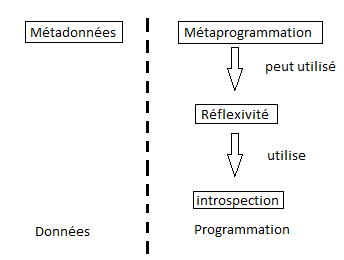
\includegraphics[scale = 0.8]{articulation.png}
   \end{center}
  \caption{Articulation entre les différents concepts vus}
\end{figure}

\normalsize{
Nous avons décide de faire la distinction entre la métaprogrammation et les métadonnées, la raison principale de ce choix est le fait que même si elles peuvent être liées et que la métaprogrammation peut utiliser les métadonnées, il s'agit de domaines bien différents et indépendants. dans la plupart des cas les métadonnées sont utilisées telles qu'elles. On peut traiter de données hors du cadre informatique/programmation. C'est donc pour cela que les métadonnées sont isolées dans le schéma ci-dessus. 
}

\section{L'ingénierie des modèles}

\normalsize{
La définition générique de l'ingénierie dirigée par les modèles selon Wikipédia est la suivante. \\

"L'ingénierie dirigée par les modèles (IDM) est le domaine de l'informatique mettant à disposition des outils, concepts et langages pour créer et transformer des modèles." \\

L'université de Brest propose une définition plus concrète. \\

"L'ingénierie dirigée par les modèles ( MDE : Model Driven Engeneering) est un paradigme de développement logiciel selon lequel l'objet de réflexion central du processus de développement est le modèle : l'idée est ici de se concentrer sur les concepts et les liens entre concepts, et ce, à divers niveaux d'abstraction, les aspects liés aux contingences d'une plateforme d'exécution cible n'apparaissant que tardivement dans le processus (comme le code source des composants par exemple). Cette approche prend tout son sens dans le cadre des architectures logicielles dirigées par les modèles utilisant des standards tels que le MDA (Model-Driven Architecture) proposé par l'OMG, ou l'outillage EMF (Eclipse Modeling Framework) proposé par IBM. " \\

Ce qui ressort de ces deux définitions, c'est la focalisation sur les modèles. Cela permet de monter encore en abstraction par rapport à l'objet. Ce qui rend l'étude plus modulable et plus axée sur un aspect, une fonctionnalité du problème à résoudre. Cette démarche est le prolongement des tentatives d'abstraction de l'architecture, du système d'exploitation puis enfin du langage. Le but final de l'ingénierie des modèles est l'universalité, ce qui pousse à comprendre le "pourquoi" d'un problème avant de faire le "comment".
}

\chapter{L'existant}

\section{Les annotations java}

\normalsize{
Les annotations Java ont été introduites en 2002 à travers le JCP (JSR-175) et ont été approuvées en septembre 2004. Les annotations sont disponibles avec le JDK version 1.5. Elles ont été introduites en tant qu'alternative aux fichiers de configuration XML. Elles reprennent la syntaxe de la Javadoc (présence de @).
Les annotations peuvent être traité de deux manières, la première à la compilation, donne des directives au compilateur. L'exemple le plus connu est @SuppressWarnings qui permet de supprimer les warnings de compilation (Une exception non traité par exemple). La deuxième manière d'utilisation des annotations est lors de l'exécution comme c'est le cas dans plusieurs API comme JPA (Persistance).\\
La partie la plus intéressante dans les annotations Java est la création d'annotation personnalisé. \\
}

\normalsize{
Tout d'abord il existe deux types d'annotation personnalisée, les "mono-arguments" et celles qui en possèdent plusieurs. La seule différence se fera lors de l'appel de l'annotation. Voici un exemple de création d'annotation. \\
}

\begin{lstlisting}[language=Java]
@Retention(RetentionPolicy.RUNTIME)
@Inherited
public @interface MonAnnotation {
    String   arg1();
    String[] arg2();
    String   arg3();
}
\end{lstlisting}

\normalsize{
On a donc d'après le code ci-dessus une annotation prenant trois paramètres arg1,arg2,arg3. L'annotation {\verb @Retention} indique que l'annotation sera conservé jusqu'à l'exécution. L'annotation {\verb @Inherited} indique que l'annotation sera conservé dans les sous-éléments (spécialisation...). L'exemple suivant montre comment est "appelée" une annotation. \\ 

\begin{lstlisting}[language=Java]
@MonAnnotation(arg1="valeur1", arg2="valeur2", arg3="valeur3")
public class MaCLasse {
 ...
}
\end{lstlisting}

\normalsize{
A ce stade là, l'annotation utilisé ne sert à pas grand chose. Pour tirer toute la puissance des annotations, il faut les exploiter. En utilisant apt, pour annotation processing tool, un dérivé un peu particulier de javac. L'explication de son implémentation étant fastidieuse, voici un lien qui explique en détail l'utilisation d'apt. \\
http://jmdoudoux.developpez.com/cours/developpons/java/chap-annotations.php\#annotations-7 \\


\section{La RTTI (Run Time Type Interface)}

\normalsize{
La RTTI (Run Time Type Interface) a été considéré à tord comme une tare du C++. En effet on disait qu'elle ralentissait les programmes, qu'elle alourdissait les binaires, et qu'elle servait à rien. D'ailleurs Coplien a dit : "il est absolument impensable que les programmeurs puissent savoir au cours de l'exécution à quels types d'objets ils ont affaire". Le but de la RTTI est d'ajouter des informations aux classes pour le programme puisse l'inspecter. Donc cela permet un mécanisme d'introspection du programme. La RTTI est souvent utiliser qu'à des fins de diagnostics ou pour éviter des erreurs de logiques dans les programmes. Voici un exemple d'utilisation de la RTTI.
}


\begin{lstlisting}[language=C++]
class A {};
class B1 : public A {};
class B2 : public B {};

...

void uneFonc()
{
   A * b1 = new B1();
   B1  b11;
   A * b2 = new B2();

   if (type_id(b1) == type_id(B1)); //Le test sera bon

   if (type_id(b1) == type_id(b11)); //Le test sera bon

   if (type_id(b1) == type_id(b2)); //Le test ne sera pas bon
	   
}
\end{lstlisting}

\normalsize{
Désormais, La RTTI est intégré par défaut à g++ depuis la version 2.8 (env. 1999) et à VC 8.0 (compilateur visual studio) 
}

\normalsize{
Le C++ de par sa conception est très différent du Java (machine virtuelle le tout objet etc) est en retard sur les notions vues précédemment. Néanmoins, on pourrait imaginer des routines pré-processeur qui pourrait analyser des "annotations" écrites à partir de \#<commande>, on pourrait ainsi très facilement imiter les annotations classiques de Java (@Override @Deprecated etc...). Pour ce qui est de la réflexion en C++ (Standard), la tâche s'annonce plus complexe, mais un mécanisme à la RTTI (informations dans l'exécutable) pourrait être exploitable pour pouvoir modifié le comportement du programme en cours d'exécution. L'annotation C++ existe déjà avec Microsoft ( http://msdn.microsoft.com/fr-fr/library/ms182032\%28v=VS.80\%29.aspx) qui propose des annotations pour réduire le risque d'erreurs de code. On a fixé l'étude au C++ standard, car en effet le C++/CLI (variante de Microsoft) prend en charge la réflexivité via le framework .NET. On peut pas retenir cette solution car l'utilisation de .NET indique que le code est exécuté à partir d'une machine virtuelle à l'instar de Java. \\
La réflexion a fait partie des domaines d'étude de la normes C++11 mais elle a pas été retenu. On peut espérer que cela reviendra très tôt à l'ordre du jour. 
}

\section{Équivalences dans les autres langages}

\normalsize{
Comme dit dans la définition de la réflexivité, il existe de nombreux langages permettant de réaliser cette fonction. Cependant, que ce soit dans l'architecture (machine virtuelle) et dans les perspectives d'avenir le C\# est l'alternative la plus ressemblante au java. En effet, L'API System.Reflection permet de produire tous les mécanismes vues précédemment mais il peut  en plus de désassembler un exécutable réalisé avec la plateforme .Net pour obtenir son architecture. On peut rapidement imaginer un métaprogramme qui puisse analyser des exécutables .NET pour effectuer des statistiques logicielles ou pour extraire le modèle UML. 
}

\chapter{Un cas concret}

\section{Étude de l'article proposé}

\normalsize{
L'article scientifique de Nicolas Dumoulin traite de la création d'interface graphique en Java à l'aide des annotations et de la Java Reflection API. \\

Dans le cas ici, Les annotations sont utilisées à des fins descriptives dans le but d'analyser l'objet étudié et observé. Le fait qu'une classe soit annoté, elle devient observable. On détaillera par la suite comment cela est utilisé.  Voici un exemple du type d'annotation qui peut être utilisé pour décrire un membre d'une classe.
}

\begin{lstlisting}[language=Java]
public class Individual {

   @Observable (description = "age in weeks")
   private short age;
}
\end{lstlisting}

\normalsize{
Ces annotations sont ensuite analyser à l'aide de l'API Java Reflection. Les types de données supportés sont les types natif de Java (int,char, float etc...) ainsi que des types classiques (Java.IO.File etc). Chaque élément annoté est transformé en composant graphique. Les descriptions sont utilisées pour donner un nom affichable qui ne soit pas soumis aux règles syntaxiques du Java (Présence d'espace, caractères spéciaux, etc...) . L'une des améliorations futures du projet est d'augmenter le nombre d'objets compatibles.   
}

\normalsize{
L'article nous montre aussi les bénéfices du développement d'une architecture dirigée par les modèles compatible avec le IBM Modeling Framework. L'auteur cite plusieurs voies concernant l'approche de l'utilisation de l'ingénierie des modèles. En effet, Microsoft propose le concept de "Software factories" pour implémenter l'approche dirigé par les modèles et IBM propose le Eclipse Modeling Framework.
}

\normalsize{
L'auteur généralise le principe de métaprogramme dans la section 4.3. Et que la plupart des développeurs seraient gagnant à utiliser ces méthodes de programmation. Il cite l'exemple de génération automatique de GUI qui fait gagner un temps de développement considérable par rapport à une écriture manuelle du code. \\
}

\normalsize{
En conclusion de cet article, Nicolas Dumoulin souligne la simplicité d'utilisation des annotations Java qui permette des des applications intéressantes comme la génération automatique d'interface graphique.
}
\chapter{Conclusion}

\normalsize{
Ce TP a été l'occasion de découvrir une couche d'abstraction supplémentaire du génie logiciel. Et par la même occasion, nous faire prendre du recul par rapport à notre conception du développement. \\
}

\normalsize{
Les divers concepts étudiées semblent être les éléments qui seront porteurs dans le génie logiciel. En effet beaucoup d'entreprises mises sur l'ingénierie des modèles et sur la métaprogrammation comme technique du futur. \\
}

\normalsize{
On peut résumer l'ingénierie des modèles, à la réflexion sur des concepts et comment les relier afin de passer outre les spécificités d'un langage ou d'une architecture. \\
} 

\normalsize{
Pour aller plus loin, ce TP nous a permis de voir nos langages de programmation usuel (C++, Java, C\#) sous d'autres formes afin d'en détecter les forces et les faiblesses potentielles et ce qui pourrait être une future évolution.
 }
\end{document}